\chapter[Extracci\'on de pigmentos vegetales y cromatograf\'ia]{Clorofila}

\begin{Huge}
	\begin{center}
		\textbf{Extracci\'on de pigmentos vegetales y cromatograf\'ia}
	\end{center}
\end{Huge}

\section{Introducci\'on}

Los mayores pigmentos fotosint\'eticos son la clorofilas, carotenoides, y ficobilinas. Entre ellos, las clorofilas y los carotenoides son los pigmentos m\'as abundantes en las hojas de las plantas superiores y otros organismos fotosint\'eticos. Las microalgas son una fuente importante de colorantes naturales, como la ficocianina, ficoeritrina, y astaxantina, que están ganando un mayor interés que los colorantes sintéticos debido a sus características no tóxicas y no cancerígenas. La ficocianina y la ficoeritrina son pigmentos fotosintéticos de color azul y rojo, respectivamente, que se encuentran en microalgas, cianobacterias, rodofitas y criptofitas.

Las clorofilas son los pigmentos que dan a las plantas su color verde caracter\'istico. Constituyen aproximadamente el 4\% del cloroplasto (en peso seco). La clorofila\textit{-b} (Chl\footnote{Chl, de la palabra en inglés "chlorophyll"} a) se presenta como un tercio del contenido de la clorofila\textit{-a}. Por lo tanto, la clorofila\textit{-a} (Chl b) es un componente de los centros de reacción fotosintéticos y podemos considerarla como el pigmento fotosintético esencial. 

La Chl a muestra dos bandas de absorción principales: una en el rojo, con un máximo alrededor de 660 nm y un pico de absorción importante en el extremo azul a violeta del espectro visible (máximo alrededor de 435 nm). La Chl b muestra también dos bandas de absorción importantes: una en el rojo-naranja del espectro visible, con un máximo a 650 nm, y la otra en el rango del azul.

\subsection{Principio}

Los pigmentos fotosint\'eticos son solubles en diferentes solventes org\'anicos. Con base a las diferencias de solubilidad de esos pigmentos en diferentes solventes, ellos pueden ser separados e identificados. 

\section{Objetivo general}

Extraer los pigmentos fotosint\'eticos presentes en las hojas de plantas herbáceas y separarlos por el m\'etodo de cromatograf\'ia.

\section{Objetivos espec\'ificos}

\begin{enumerate}
	\item Extracci\'on de pigmentos fotosint\'eticos de hojas de lechuga y espinaca.
	\item Comparar los pigmentos extra\'idos con cromatograf\'ia de papel.
\end{enumerate}

\section{Materiales}

\subsection{Material requerido}

\begin{enumerate}
	\item Medio litro de alcohol isopropílico 
	\item Dos vasos de vidrio con tapa
	\item Dos morteros con pistilo
	\item Dos lapices
	\item Dos filtros para caf\'e
	\item Dos vasos de precipitado de 500 mL
	\item Una cinta adhesiva
\end{enumerate}

\subsection{Material por grupo}

\begin{enumerate}
	\item Parrilla de calentamiento
	\item Un vaso de precipitado de 1 L
\end{enumerate}

\section{Metodolog\'ia}

\subsection{Preparar reactivos}

Poner a calentar un litro de agua en la parrilla de calentamiento y los filtros para caf\'e recortarlos en tiras de dos cent\'imetros de ancho y el largo debe ser unos tres cent\'imetros mayor que la altura del vaso de vidrio.

\subsection{Procedimiento}

Tomar unas hojas y triturarlas en el mortero hasta dejar una pasta. Luego vamos a colocar dicha pasta en el vaso de vidrio y agregamos alcohol isoprop\'ilico hasta cubrirlo. Cerramos muy bien el vaso y lo colocamos dentro de un vaso de precipitado de 500 mL, posteriormente agregamos agua caliente. Dejarlo por lo menos media hora y si el agua se enfr\'ia podemos reemplazarla para mantener la temperatura del agua caliente.

A continuaci\'on, retiramos el vaso de vidrio y quitamos la tapa. Con la cinta adhesiva pegamos una tira de papel al l\'apiz y lo colocamos sobre el vaso de vidrio(ver figura~\ref{fig:cromatografia}). De est\'a manera la cinta quedar\'a dentro del vaso y la parte inferior de la tira estar\'a sumergida en el alcohol isopropílico entre una o dos horas.

Al terminar le puedes tomar una fotograf\'ia con tu celular o c\'amara fotogr\'afica. Para presentar la diferencia de colores entre las cromatograf\'ias de las hojas de lechuga y espinaca vamos utilizar el sistema RGB. El modo de color RGB ("Red", "Green", y "Blue") es la composici\'on de los colores primarios en funci\'on de su intensidad. Por lo general, la intensidad de cada uno de los componentes se encuentran en una escala de 0 a 255. Por ejemplo, los colores de la UNAM son azul (RGB: 0, 61, 121) y oro (RGB: 213, 159, 15). En algunos casos se puede agregar un cuarto valor que representa la transparencia. 

Para conocer los colores en el sistema RGB deben subir su fotograf\'ia a la pagina web https://imagecolorpicker.com/ y seguir los siguientes pasos:

\begin{enumerate}
	\item Abrir la pagina https://imagecolorpicker.com/ 
	\item Dar clic en \textbf{Use Your Image} para cargar la imagen
	\item Poner el cursor sobre la imagen y dar clic en la parte que necesitamos conocer su color en t\'erminos de RGB
	\item Copiar los primeros tres valores 
\end{enumerate}


\begin{figure}[h]
	
	\begin{leftbar}
		
		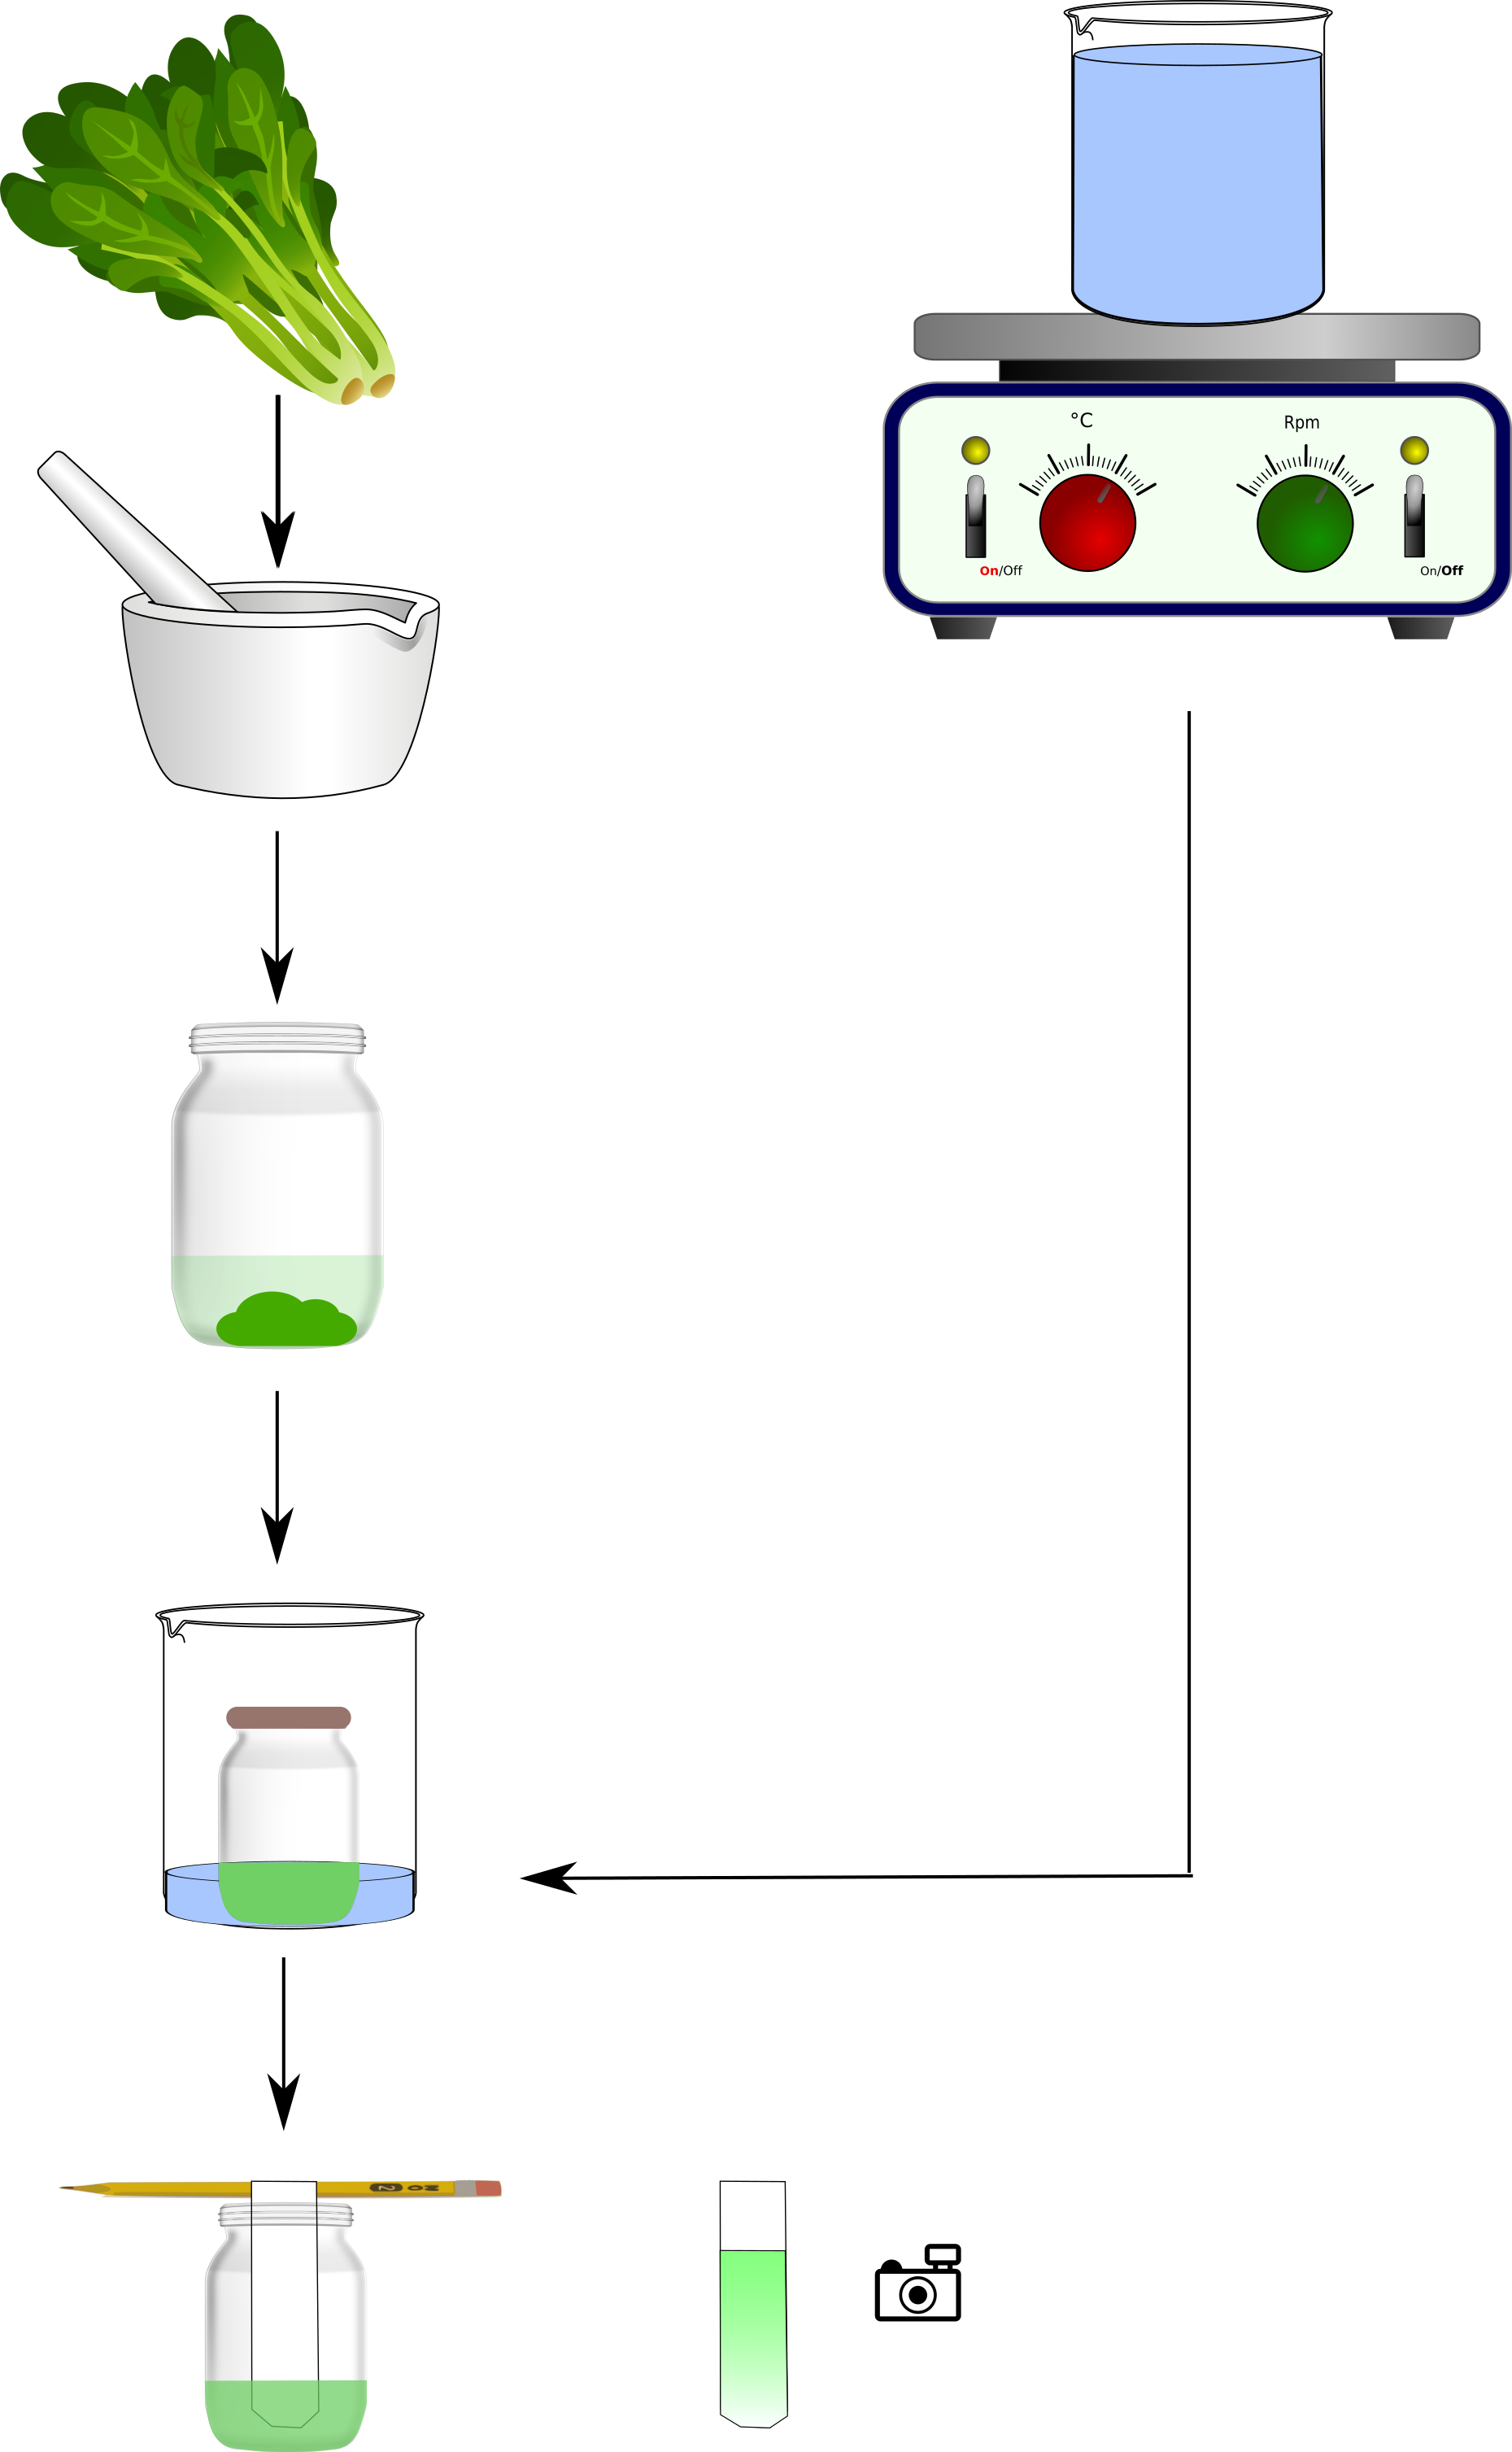
\includegraphics[width=0.5\textwidth]{cromatofrafia.png}
		\centering
		\caption{\textit{Procedimiento para extraer los pigmentos fotosint\'eticos presentes en las hojas de las plantas y separarlos por el m\'etodo de cromatograf\'ia.}}
		\label{fig:cromatografia}
		
	\end{leftbar}
	
\end{figure}

\section{Resultados}

Presentar las fotograf\'ias y sus valores respectivos en el sistema RGB

\section{Cuestionario}

\begin{enumerate}
	\item \textquestiondown Por qu\'e la clorofila es verde?
	\item \textquestiondown Por qu\'e la clorofila \textit{-a} es m\'as abundante?
	\item La energ\'ia de la luz irradiada es inversamente proporcional a la longitud de onda. \textquestiondown verdadero o falso?
	\item \textquestiondown Cu\'al es la importancia de la expresi\'on anterior, con respecto al pico de absorción de la  clorofila \textit{-a}?
	\item \textquestiondown Cu\'al planta cree usted que present\'o una mayor cantidad de clorofila en sus hojas?
\end{enumerate}


